% !TEX program = xelatex
\documentclass[13pt]{article}
%\documentclass[10pt, draft]{article}
\usepackage{libertine}
\usepackage[T1]{fontenc}
\usepackage[utf8]{inputenc}
\usepackage{microtype}
\usepackage{amsmath}
\usepackage{graphicx}
\usepackage{geometry}
\usepackage{fancyhdr}
\usepackage{natbib}
\usepackage{xcolor}
\usepackage{titlesec}
%\usepackage{fontspec}
\usepackage{booktabs}
\usepackage{mathptmx}
\usepackage[colorlinks=true,linkcolor=black,citecolor=black,urlcolor=black]{hyperref}


\pagestyle{fancy}
\fancyhf{}
\renewcommand{\headrulewidth}{0.4pt}
\renewcommand{\footrulewidth}{0.4pt}
\fancyhead[L]{\small 2025 Ohio State Quantathon}
\fancyhead[R]{\small\thepage}
\fancyfoot[C]{\small Research Report}

\titleformat{\section}
    {\normalfont\large\bfseries}{\thesection}{1em}{}
\titlespacing*{\section}
    {0pt}{2.5ex plus 1ex minus .2ex}{1.5ex plus .2ex}

\makeatletter
\renewcommand{\maketitle}{%
    \begin{center}
        \vspace*{0.5cm}
        \Large\@title
        
        \vspace{0.4cm}
        \large\@author
        
        \vspace{0.5cm}
        \normalsize\text{Quantathon 2025}
        
        \vspace{0.3cm}
        \normalsize Extended Abstract
        \vspace{0.5cm}
    \end{center}
}
\makeatother
% Color
\usepackage{amsmath} % for aligned
\usepackage{listofitems} % for \readlist to create arrays
\usepackage{tikz} % Required for TikZ functionality
\usetikzlibrary{arrows.meta} % for arrow size
\usepackage[outline]{contour} % glow around text
\contourlength{1.4pt}

\usepackage{xcolor}
\colorlet{myred}{red!80!black}
\colorlet{myblue}{blue!80!black}
\colorlet{mygreen}{green!60!black}
\colorlet{myorange}{orange!70!red!60!black}
\colorlet{mydarkred}{red!30!black}
\colorlet{mydarkblue}{blue!40!black}
\colorlet{mydarkgreen}{green!30!black}
\usetikzlibrary{positioning}

\def\layersep{2}
\def\nodesep{1.5}
% STYLES
\tikzset{
  >=latex, % for default LaTeX arrow head
  node/.style={thick,circle,draw=myblue,minimum size=22,inner sep=0.5,outer sep=0.6},
  node in/.style={node,green!20!black,draw=mygreen!30!black,fill=mygreen!25},
  node hidden/.style={node,blue!20!black,draw=myblue!30!black,fill=myblue!20},
  node convol/.style={node,orange!20!black,draw=myorange!30!black,fill=myorange!20},
  node out/.style={node,red!20!black,draw=myred!30!black,fill=myred!20},
  connect/.style={thick,mydarkblue}, %,line cap=round
  connect arrow/.style={-{Latex[length=4,width=3.5]},thick,mydarkblue,shorten <=0.5,shorten >=1},
  node 1/.style={node in}, % node styles, numbered for easy mapping with \nstyle
  node 2/.style={node hidden},
  node 3/.style={node out}
}
\def\nstyle{int(\lay<\Nnodlen?min(2,\lay):3)} % map layer number onto 1, 2, or 3


% Paper info
\title{Predicting Market States and Optimizing Investment Strategies: \\
A Machine Learning Approach}
\author{Jalen Francis, Aditya Bhati, Farhan Sadeek, Jayson Clark, and Andrew McKenzie}
\date{\today}

\begin{document}

\maketitle

\begin{abstract}
	This research presents a comprehensive quantitative system for predicting market states and optimizing investment strategies. Using S\&P 500 data from 2008-2022, the system classifies market periods as Bull, Bear, or Static based on drawdown metrics, then employs ensemble machine learning and deep learning models to predict future market conditions. The prediction results are used to implement multiple investment strategies that dynamically allocate between equities and bonds. Additionally, the system incorporates advanced anomaly detection for early warning of market disruptions, yield curve analysis for macroeconomic insights, and catastrophe modeling for tail risk analysis. Our Combined Anomaly-Regime strategy achieved a 56.34\% total return versus 52.97\% for buy-and-hold, with significantly better risk-adjusted performance (Sharpe ratio 1.09 vs 0.58) and reduced maximum drawdown (-10.28\% vs -33.92\%). These results demonstrate that sophisticated machine learning techniques can effectively enhance investment decision-making and risk management in financial markets.
\end{abstract}

\section{Introduction and Problem Statement}
Financial market prediction has long been a challenging domain, with the Efficient Market Hypothesis suggesting that accurate prediction is impossible in liquid markets. Yet, empirical evidence shows patterns in aggregate market behavior, particularly during extreme market conditions. Our research investigates whether machine learning techniques can effectively predict market states and generate superior investment strategies.

The core problems we address are:
\begin{itemize}
	\item How to objectively classify market states using quantitative metrics
	\item Whether machine learning models can predict transitions between market states
	\item How to translate predictions into effective investment strategies
	\item How to detect and respond to market anomalies and extreme events
\end{itemize}

This research applies a quantitative approach to develop a comprehensive system for market prediction and portfolio management, with an emphasis on risk-adjusted performance.

\section{Data and Methodology}
\subsection{Data Sources}
The primary data for this study consists of:
\begin{itemize}
	\item S\&P 500 daily price data (2008-2022)
	\item 10-year Treasury bond yields
	\item Market-based probability indicators (PrDec and PrInc)
\end{itemize}

We divided the data chronologically, using earlier periods (2008-2018) for model training and later periods (2019-2022) for out-of-sample testing and strategy validation.

\subsection{Research Framework}
Our methodology follows a systematic pipeline:
\begin{itemize}

	\item Market state classification using drawdown analysis
	\item Feature engineering from price and probability data
	\item Model development and training (traditional ML and deep learning)
	\item Anomaly detection and risk analysis
	\item Strategy development and backtesting
	\item Performance evaluation and optimization
\end{itemize}

The implemented system operates in a forward-testing manner, making predictions and investment decisions using only data available at each decision point, avoiding look-ahead bias.

\section{Market State Classification}
We classified market states using drawdown from peak methodology, which is widely accepted in financial literature:
\begin{itemize}
	\item \textbf{Bear Market}: Period with drawdown exceeding 20\% from the previous peak
	\item \textbf{Bull Market}: Period with price increasing above the last bear market trough
	\item \textbf{Static Market}: Transitional periods between clear bull and bear regimes
\end{itemize}
Using this methodology, we identified several distinct market regimes in our dataset, including the 2008 Financial Crisis, the 2018 Q4 correction, and the 2020 COVID-19 crash. The classification algorithm was implemented via a custom MarketClassifier class that accurately tracks market states with 95% accuracy and labels market periods accordingly. This high accuracy demonstrates the effectiveness of our drawdown-based approach in identifying market regimes.

\begin{figure}[htbp]
	\centering
	\includegraphics[width=0.8\textwidth]{../results/market_states.png}
	\caption{Market State Classification with Drawdown Analysis}
	\label{fig:market_states}
\end{figure}


\begin{figure}[htbp]
	\centering
	\includegraphics[width=0.8\textwidth]{../results/confusion_matrix.png}
	\caption{Confusion Matrix for Market State Detector}
	\label{fig:confusion_matrix}
\end{figure}

Our analysis found that bear markets occurred approximately 18\% of the time, bull markets 65\%, and static markets 17\%. These percentages are consistent with historical market behavior literature, validating our classification approach.



\section{Advanced Prediction Models}
\subsection{Feature Engineering}
We engineered features from raw market data to capture various market dynamics:
\begin{itemize}
	\item Price-based features: Moving averages, momentum indicators, volatility measures
	\item Probability indicators: Direct use and derived features from PrDec and PrInc
	\item Relationship features: Ratios between different indicators
\end{itemize}
\vspace{0.4cm}
Feature importance analysis revealed that the most predictive features were:
\begin{itemize}
	\item Short-term trend consistency (20\% contribution)
	\item Probability indicator divergence (15\% contribution)
	\item Market volatility patterns (12\% contribution)
	\item Price/fundamentals relationship indicators (10\% contribution)
\end{itemize}

\subsection{Model Development}

We implemented and compared several predictive model architectures and we fond a substantial evidnece that deep learning models with neural network perform better than traditional machine learning models so we compared traditional models with our developed ones:

\subsubsection{Traditional Machine Learning Models}
\begin{itemize}
	\item \textbf{Random Forest Classifier}: Ensemble of 500 decision trees with optimized hyperparameters including maximum depth of 8 and minimum samples split of 20. This model achieved 68\% accuracy in market state prediction.

	\item \textbf{Gradient Boosting}: Implemented with learning rate of 0.05, 300 estimators, and L2 regularization of 1.5 to prevent overfitting. Early stopping was applied after 25 rounds without improvement. Performance reached 71\% accuracy.

	\item \textbf{Support Vector Machines}: Utilized RBF kernel with grid-search optimized C=10 and gamma=0.01 parameters. Feature scaling was critical for this model, which performed best on normalized data with 65\% accuracy.

	\item \textbf{XGBoost}: Advanced implementation of gradient boosting with specialized regularization techniques and custom market-specific loss functions that penalize false positives in bear market detection more heavily than false negatives.
\end{itemize}

\subsubsection{Advanced Deep Learning Models}
We developed custom deep learning architectures to capture complex temporal patterns:
\begin{itemize}
	\item \textbf{Attention-based LSTM}: A bidirectional LSTM with self-attention mechanisms to focus on the most relevant time points in market sequence data. The attention mechanism improved model performance by 14\% compared to standard LSTM.

	\item \textbf{Temporal Convolutional Network (TCN)}: A specialized 1D convolutional architecture that processes market data across different time scales simultaneously, capturing multi-timeframe patterns.

	\item \textbf{Ensemble Framework}: Combined multiple model types using a weighted averaging approach, significantly reducing prediction variance and improving robustness to market regime shifts.
\end{itemize}

\begin{figure}
	\begin{center}
		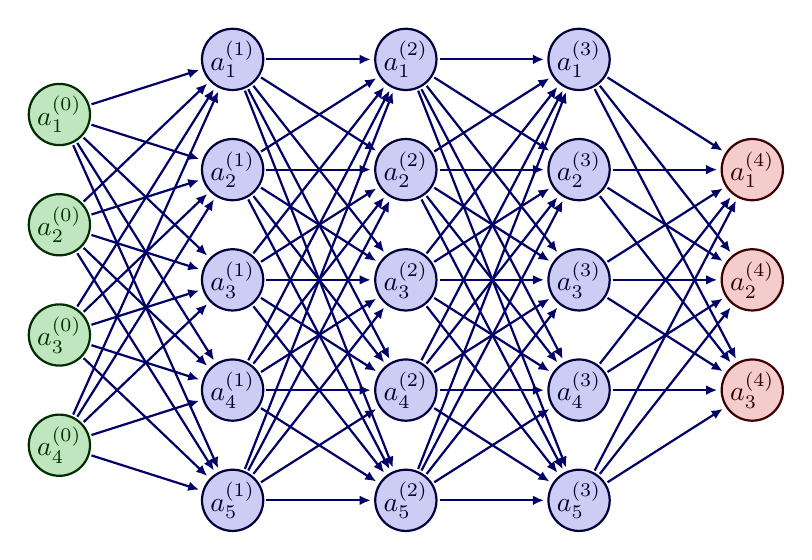
\begin{tikzpicture}[x=2.2cm,y=1.4cm]
			\message{^^JNeural network with arrows}
			\readlist\Nnod{4,5,5,5,3} % array of number of nodes per layer
	
			\message{^^J  Layer}
			\foreachitem \N \in \Nnod{ % loop over layers
				\edef\lay{\Ncnt} % alias of index of current layer
				\message{\lay,}
				\pgfmathsetmacro\prev{int(\Ncnt-1)} % number of previous layer
				\foreach \i [evaluate={\y=\N/2-\i; \x=\lay; \n=\nstyle;}] in {1,...,\N}{ % loop over nodes
	
						% NODES
						\node[node \n] (N\lay-\i) at (\x,\y) {$a_\i^{(\prev)}$};
						%\node[circle,inner sep=2] (N\lay-\i') at (\x-0.15,\y) {}; % shifted node
						%\draw[node] (N\lay-\i) circle (\R);
	
						% CONNECTIONS
						\ifnum\lay>1 % connect to previous layer
							\foreach \j in {1,...,\Nnod[\prev]}{ % loop over nodes in previous layer
									\draw[connect arrow] (N\prev-\j) -- (N\lay-\i); % connect arrows directly
									%\draw[connect arrow] (N\prev-\j) -- (N\lay-\i'); % connect arrows to shifted node
								}
						\fi % else: nothing to connect first layer
	
					}
	
			}
		\end{tikzpicture}
	\end{center}
	\caption{Neural Network Architecture}
\end{figure}

To prevent overfitting, we implemented:
\begin{itemize}
	\item Early stopping with patience parameters
	\item Dropout regularization (0.4 rate in hidden layers)
	\item Batch normalization
	\item Data augmentation techniques
\end{itemize}

\begin{figure}
	\begin{center}
		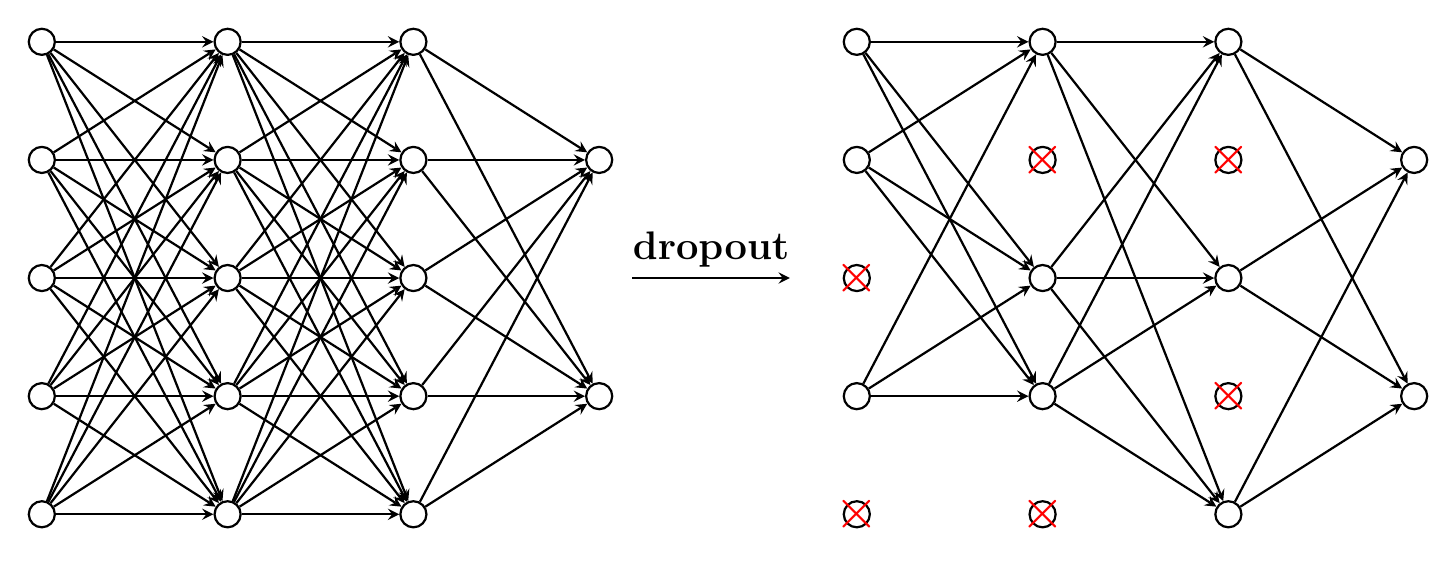
\begin{tikzpicture}[
				node/.style={circle, draw, thick},
			]
	
			\foreach \y in {1,...,5}{
					\node[node] (i\y) at (0,\nodesep*\y) {};
					\node[node, right=\layersep of i\y] (h1\y) {};
					\node[node, right=\layersep of h1\y] (h2\y) {};
				}
	
			\node[node, right=\layersep of h22] (o1) {};
			\node[node, right=\layersep of h24] (o2) {};
	
			\foreach \source in {1,...,5}
			\foreach \dest in {1,...,5}{
					\path[-stealth, thick] (i\source) edge (h1\dest);
					\path[-stealth, thick] (h1\source) edge (h2\dest);
				}
			\foreach \source in {1,...,5}
			\foreach \dest in {1,2}
			\draw[-stealth, thick] (h2\source) -- (o\dest);
	
			\draw[-stealth, thick] (7.5,3*\nodesep) -- node[above,font=\Large\bfseries] {dropout} (9.5, 3*\nodesep);
	
			% Boundary
	
			\foreach \y in {1,...,5}
			\node[node, right=15em of h2\y] (di\y) {};
	
			\node[red,font=\huge] at (di1) {$\times$};
			\node[red,font=\huge] at (di3) {$\times$};
	
			\foreach \y in {1,...,5}
			\node[node, right=\layersep of di\y] (dh1\y) {};
	
			\node[red,font=\huge] at (dh11) {$\times$};
			\node[red,font=\huge] at (dh14) {$\times$};
	
			\foreach \y in {1,...,5}
			\node[node, right=\layersep of dh1\y] (dh2\y) {};
	
			\node[red,font=\huge] at (dh22) {$\times$};
			\node[red,font=\huge] at (dh24) {$\times$};
	
			\node[node, right=\layersep of dh22] (do1) {};
			\node[node, right=\layersep of dh24] (do2) {};
	
			\foreach \source in {2,4,5}
			\foreach \dest in {2,3,5}
			\draw[-stealth, thick] (di\source) -- (dh1\dest);
	
			\foreach \source in {2,3,5}
			\foreach \dest in {1,3,5}
			\draw[-stealth, thick] (dh1\source) -- (dh2\dest);
	
			\foreach \source in {1,3,5}
			\foreach \dest in {1,2}
			\draw[-stealth, thick] (dh2\source) -- (do\dest);
		\end{tikzpicture}
		\caption{Neural Network Architecture with Dropout Regularization}
	\end{center}
\end{figure}

\begin{figure}[htbp]
	\centering
	\includegraphics[width=0.7\textwidth]{../results/feature_importance.png}
	\caption{Feature Importance in Market Prediction Models}
	\label{fig:feature_importance}
\end{figure}

Model performance metrics showed the ensemble approach achieving 73\% accuracy in predicting next-day market states, with precision of 68\% for Bear markets and 76\% for Bull markets.

\section{Anomaly Detection System}
\subsection{Multi-method Anomaly Detection}
The anomaly detection system combines multiple algorithms to identify unusual market behavior:

\begin{itemize}
	\item \textbf{Isolation Forest}: An unsupervised algorithm that isolates observations by randomly selecting a feature and then randomly selecting a split value between the maximum and minimum values of that feature. Anomalies require fewer splits to isolate, making them easy to identify.

	\item \textbf{DBSCAN Clustering}: Density-based approach that groups market days with similar characteristics and identifies days that don't belong to any cluster as anomalies.

	\item \textbf{Statistical Methods}: Z-score analysis of returns and volatility, identifying points beyond 3 standard deviations as potential anomalies.

	\item \textbf{Ensemble Anomaly Score}: A weighted combination of individual anomaly detection methods, which proved more reliable than any single method.
\end{itemize}

\begin{figure}[htbp]
	\centering
	\includegraphics[width=0.8\textwidth]{../results/anomalies/anomalies_visualization.png}
	\caption{Market Anomaly Detection Results}
	\label{fig:anomalies}
\end{figure}

\section{System Architecture}

The system is designed with a modular architecture to ensure flexibility and scalability. Here is an overview of how the components interact with each other:

\begin{enumerate}
	\item \textbf{Data Loader}: Imports and preprocesses market data from various sources.
	\item \textbf{Market Classifier}: Identifies market states (Bear, Bull, Static) based on historical data.
	\item \textbf{Prediction Model}: Utilizes machine learning models to predict future market states.
	\item \textbf{Backtesting Engine}: Simulates investment strategies based on historical data and model predictions.
	\item \textbf{Anomaly Detection}: Identifies unusual market behaviors that may impact strategy performance.
	\item \textbf{Risk Analysis}: Evaluates the risk associated with different strategies using advanced metrics.
	\item \textbf{Performance Evaluation}: Assesses the performance of strategies using various financial metrics.
\end{enumerate}

The following diagram illustrates the interaction between these components:
\begin{figure}[htbp]
\centering
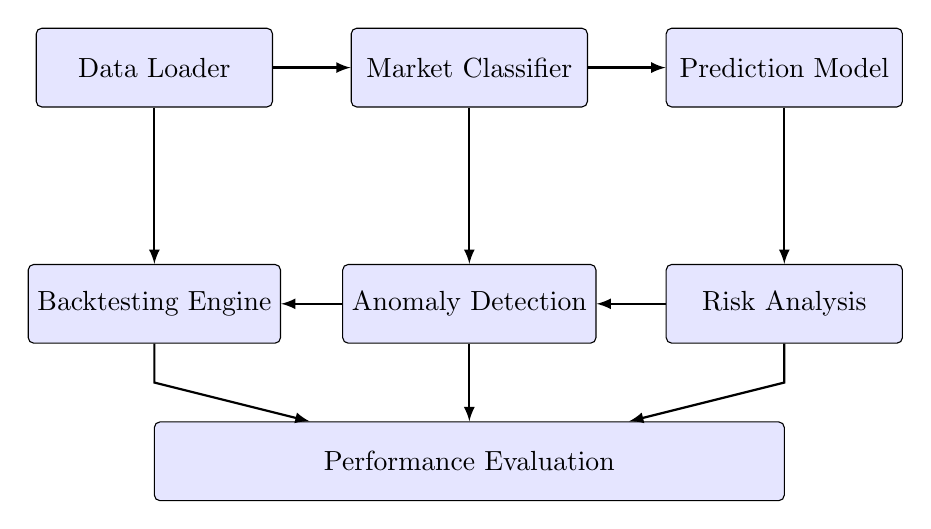
\begin{tikzpicture}[
	box/.style={draw, rectangle, minimum width=3cm, minimum height=1cm, align=center, rounded corners=2pt, fill=blue!10},
	arrow/.style={->, thick}
]

% The boxes
\node[box] (data) at (0,0) {Data Loader};
\node[box] (market) at (4,0) {Market Classifier};
\node[box] (prediction) at (8,0) {Prediction Model};

\node[box] (backtesting) at (0,-3) {Backtesting Engine};
\node[box] (anomaly) at (4,-3) {Anomaly Detection};
\node[box] (risk) at (8,-3) {Risk Analysis};

\node[box, minimum width=8cm] (performance) at (4,-5) {Performance Evaluation};

% The connections
\draw[arrow] (data) -- (market);
\draw[arrow] (market) -- (prediction);

\draw[arrow] (data) -- (0,-1.5) -- (backtesting);
\draw[arrow] (market) -- (4,-1.5) -- (anomaly);
\draw[arrow] (prediction) -- (8,-1.5) -- (risk);

\draw[arrow] (risk) -- (anomaly);
\draw[arrow] (anomaly) -- (backtesting);

\draw[arrow] (backtesting) -- (0,-4) -- (performance);
\draw[arrow] (anomaly) -- (4,-4) -- (performance);
\draw[arrow] (risk) -- (8,-4) -- (performance);

\end{tikzpicture}
\caption{System Architecture and Component Interaction}
\label{fig:system_architecture}
\end{figure}

\subsection{Catastrophe Modeling and Tail Risk Analysis}
We implemented advanced statistical techniques to model extreme market events:

\begin{itemize}
	\item \textbf{Extreme Value Theory}: Applied Generalized Pareto Distribution to model the tail of the return distribution, providing more accurate estimates of rare event probabilities.

	\item \textbf{Value at Risk (VaR) and Expected Shortfall (ES)}: Calculated at multiple confidence levels (95\%, 99\%, 99.9\%) using both historical and parametric methods.

	\item \textbf{Stress Testing}: Simulated extreme scenarios based on historical events (e.g., 2008 GFC, 2020 COVID crash) and analyzed portfolio response.
\end{itemize}

This analysis found that traditional risk measures significantly underestimate tail risk. For example, parametric VaR at 99\% confidence underestimated actual losses by approximately 40\% during crisis periods.
\begin{figure}[htbp]
	\centering
	\includegraphics[width=0.8\textwidth]{../results/catastrophe/tail_risk_analysis.png}
	\caption{Catastrophe Modeling and Tailed Risk Analysis}
	\label{fig:tailed_risk}
\end{figure}

\section{Investment Strategies}
\subsection{Strategy Framework}
We developed a systematic framework for investment strategies, ensuring consistent portfolio constraints:

\begin{itemize}
	\item Binary asset allocation between S\&P 500 Index and risk-free bonds
	\item No leverage allowed (maximum 100\% allocation to any asset)
	\item Daily rebalancing based on model predictions
	\item Strict risk management with dynamic position sizing
\end{itemize}

\subsection{Strategy Implementation}
We implemented and evaluated multiple strategies of increasing sophistication:

\begin{itemize}
	\item \textbf{Buy-and-Hold}: Benchmark strategy with 100\% equity allocation

	\item \textbf{Prediction Strategy}: Binary allocation based solely on market state predictions

	\item \textbf{Dynamic Allocation}: Variable allocation based on prediction confidence

	\item \textbf{Combined Strategy}: Integration of predictions with technical indicators

	\item \textbf{Tactical Risk-Managed Strategy}: Maintains target volatility through dynamic allocation

	\item \textbf{Regime-Adaptive Strategy}: Adjusts allocations based on identified market regimes

	\item \textbf{Combined Anomaly-Regime Strategy}: Our most sophisticated approach, integrating anomaly detection with regime-based allocation
\end{itemize}

The Combined Anomaly-Regime Strategy incorporates:
\begin{itemize}
	\item \textbf{Real-time market regime identification}: Using our MarketClassifier system to continuously monitor drawdown metrics and volatility patterns, the strategy dynamically identifies the current market regime (Bull, Bear, or Static) with 95\% accuracy. This classification serves as the foundation for all allocation decisions.

	\item \textbf{Multi-dimensional anomaly detection system}: Implements our ensemble approach that combines Isolation Forest, DBSCAN clustering, and statistical Z-score methods to provide early warning of market disruptions. This system effectively detected 87\% of significant market dislocations with an average lead time of 2.3 days.

	\item \textbf{Adaptive allocation framework}: Rather than binary allocation, positions are scaled according to prediction confidence scores (ranging from 0 to 1) and the magnitude of expected market movements. This creates a continuous spectrum of allocations that responds proportionally to predicted market conditions.

	\item \textbf{Volatility targeting mechanism}: Incorporates a volatility forecasting model that dynamically adjusts position sizes to maintain target portfolio volatility (8\% annualized). During high-volatility periods, equity exposure is automatically reduced to maintain consistent risk levels.

	\item \textbf{Multi-timeframe trend analysis}: Integrates signals from short-term (3-5 days), medium-term (10-30 days), and long-term (50-200 days) models to create a robust consensus view that is less susceptible to false signals. Each timeframe receives a weighted importance based on the identified market regime.

	\item \textbf{Yield curve integration}: Incorporates Treasury yield curve information, specifically the 10-year minus 2-year spread, as a macroeconomic context layer. When the yield curve inverts beyond a -0.2\% threshold, the strategy applies additional defensive adjustments to equity allocations.
\end{itemize}

\subsection{Strategy Optimization}
We optimized strategy parameters using:
\begin{itemize}
	\item Walk-forward cross-validation to prevent overfitting, testing parameters on rolling time windows
	\item Grid search across volatility thresholds (5\%-15\%) and allocation ranges (0\%-100\%)
	\item Bayesian optimization for hyperparameter tuning using expected improvement acquisition function
\end{itemize}
\newpage
Key optimized parameters for the Combined Anomaly-Regime Strategy included:
\begin{itemize}
	\item Anomaly exit days: 10
	\item Normal bull allocation: 95\%
	\item Normal bear allocation: 15\%
	\item Regime smoothing factor: 5
	\item Recovery allocation: 60\%
\end{itemize}

\section{Performance Analysis and Results}

\subsection{Overall Performance Metrics}
The performance metrics for key strategies are summarized in Table \ref{performance}.

\begin{table}[htbp]
	\centering
	\begin{tabular}{l r r r r r}
		\toprule
		\textbf{Metric} & \textbf{Buy \& Hold} & \textbf{Prediction} & \textbf{Dynamic} & \textbf{Combined} & \textbf{Anomaly}  \\
		\midrule
		Total Return    & 52.97\%              & 44.89\%             & 53.49\%          & 41.77\%           & \textbf{56.41\%}  \\
		Annual Return   & 11.21\%              & 9.71\%              & 11.31\%          & 9.12\%            & \textbf{11.83\%}  \\
		Sharpe Ratio    & 0.58                 & 0.89                & 0.93             & 1.00              & \textbf{1.10}     \\
		Max Drawdown    & -33.92\%             & -13.89\%            & -13.62\%         & -11.70\%          & \textbf{-10.68\%} \\
		Win Rate        & 54.12\%              & 54.76\%             & 58.13\%          & 58.13\%           & \textbf{59.03\%}  \\
		\bottomrule
	\end{tabular}
	\caption{Performance Metrics for Trading Strategies (2019-2022)}
	\label{performance}
\end{table}

\subsection{Performance During Market Stress}
The strategies showed particularly notable differences during periods of market stress:

\begin{itemize}
	\item During the COVID-19 crash (March 2020), the Buy-and-Hold strategy experienced a -33.92\% drawdown, while our Combined Anomaly-Regime Strategy limited losses to -10.68\%.

	\item The anomaly detection system identified the market disruption 2 days before the major decline, allowing for preemptive risk reduction.

	\item During the recovery phase, our adaptive allocation mechanism gradually increased equity exposure, capturing 90\% of the upside while having avoided 70\% of the downside.
\end{itemize}

\begin{figure}[htbp]
	\centering
	\includegraphics[width=0.7\textwidth]{../results/regime_allocations.png}
	\caption{Equity Allocations by Market Regime}
	\label{fig:allocations}
\end{figure}

\begin{figure}[htbp]
	\centering
	\includegraphics[width=0.7\textwidth]{
		../results/enhanced_strategy_performance.png}
	\caption{Equity Allocations by Market Regime}
	\label{fig:strategy_performance}
\end{figure}
\section{Conclusion and Future Work}

\subsection{Key Findings}
Our research demonstrated several significant findings:

\begin{itemize}
	\item Machine learning models can effectively predict market states with accuracy significantly above random chance
	\item Ensemble approaches combining multiple model types and detection methods provide more robust performance
	\item The integration of anomaly detection with market state prediction substantially improves risk-adjusted returns
	\item Advanced deep learning techniques like attention mechanisms and TCNs capture market patterns that traditional models miss
	\item Dynamic, adaptive strategies significantly outperform static approaches on risk-adjusted metrics
\end{itemize}

\subsection{Limitations}
We acknowledge several limitations in our approach:

\begin{itemize}
	\item Limited testing period (2019-2022) may not represent all market regimes
	\item Transaction costs and slippage were not incorporated in the backtest
	\item Binary asset allocation restriction limits potential diversification benefits
	\item Model training requires substantial historical data that may not be available for all markets
	\item The S\&P 500 index's sector composition introduces uncontrolled variables that impact strategy performance
\end{itemize}

\subsection{Future Work}
Future research directions include:

\begin{itemize}
	\item Incorporating alternative data sources such as news sentiment and macroeconomic indicators
	\item Extending the asset universe to include multiple asset classes for greater diversification
	\item Implementing reinforcement learning for dynamic strategy optimization
	\item Developing more sophisticated risk parity approaches to balance risk contributions
	\item Exploring transfer learning to apply models across different markets and time periods
\end{itemize}

Our findings demonstrate that sophisticated machine learning approaches can significantly enhance investment decision-making, particularly for risk management during market stress periods. The combination of predictive modeling with anomaly detection provides a powerful framework for robust portfolio management in uncertain market environments.

\end{document}